\documentclass[12pt, twoside]{article}
\usepackage[letterpaper, margin=1in, headsep=0.5in]{geometry}
\usepackage[english]{babel}
\usepackage[utf8]{inputenc}
\usepackage{amsmath}
\usepackage{amsfonts}
\usepackage{amssymb}
\usepackage{tikz}
\usepackage{yhmath}
%\usetikzlibrary{quotes, angles}

\usepackage{graphicx}
\usepackage{enumitem}
\usepackage{multicol}

\usepackage{fancyhdr}
\pagestyle{fancy}
\fancyhf{}
\renewcommand{\headrulewidth}{0pt} % disable the underline of the header

\fancyhead[RE]{\thepage}
\fancyhead[RO]{\thepage \\ Name: \hspace{3cm}}
\fancyhead[L]{BECA / Dr. Huson / 10th Grade Geometry\\* 5 February 2020}

\begin{document}
\subsubsection*{8.7 Do Now: Area, volume, solids, circles review}
 \begin{enumerate}

  \item Find the area of the shape shown below composed of a rectangle and circular ends. Leave your answer as an exact value in terms of $\pi$.
  \begin{flushright}
  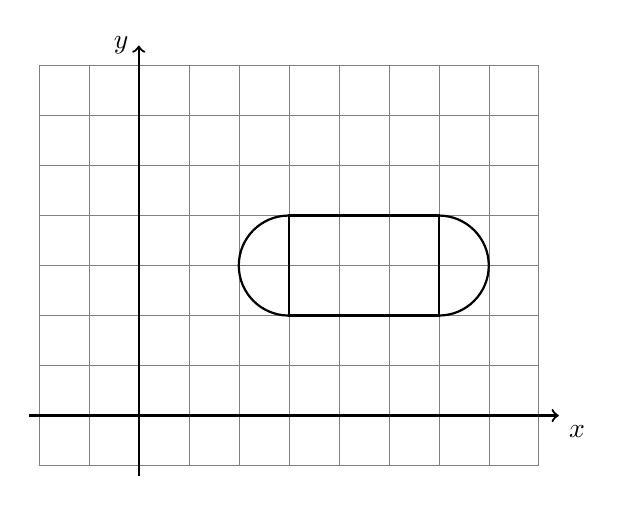
\begin{tikzpicture}[scale=.635]
    \draw [help lines] (-2,-1) grid (8,7);
    \draw [thick, ->] (-2.2,0) -- (8.4,0) node [below right] {$x$};
    \draw [thick, ->] (0,-1.2)--(0,7.4) node [left] {$y$};
    \draw [thick] (3,2)--(6,2)--(6,4)--(3,4)--cycle;
    \draw [thick] (3,4) arc (90:270:1);
    \draw [thick] (6,2) arc (-90:90:1);
  \end{tikzpicture}
\end{flushright}\vspace{1cm}

\item Perform each calculation, writing down the full calculator display and then rounding to the \emph{nearest thousandth}.
\begin{multicols}{2}
\begin{enumerate}[itemsep=2cm]
  \item $V=\frac{4}{3} \pi (10.1)^3$
  \item $P=2 \times 14.7 + \frac{1}{2} \pi (14.7)^2$  
\end{enumerate}
\end{multicols}\vspace{3cm}

\item Solve each equation for the appropriate variable. Do not round. Simplify radicals.
\begin{multicols}{2}
\begin{enumerate}[itemsep=2cm]
  \item $A=\pi r^2=20\pi$
  \item $V=\frac{1}{3}(5.25)^2h=147$  
\end{enumerate}
\end{multicols}\vspace{2cm}

\newpage
\subsubsection*{Applying density ratios}
  \item Find the weight of a plastic block with a volume of 50 cubic inches and a density of 0.15 pounds per cubic inch. \vspace{3cm}
  \item A propane tank holds 8000 cubic liters. Find the cost to completely fill the tank if propane costs \$0.12 per $l^3$. \vspace{2cm}
  \item A bar of silver is in the shape of a rectangular prism having a length of 15 cm, width of 6 cm, and thickness of 3.5 cm. The density of silver is 12.3 grams per cubic cm, and its approximate market value is \$0.90 per gram.
  \begin{enumerate}
    \item Find the weight of the bar of silver.  \vspace{3cm}
    \item Find its value in dollars.
  \end{enumerate} \vspace{2cm}

  \item A cylinder is 18.3 cm tall and has a volume of 1000 cubic cm. Find the area of the base of the cylinder. Express your result to the \emph{nearest hundredth of a square centimeter}. \vspace{3cm}


\newpage
  \item The sector $AOB$ in circle $O$ has an area of $12.8\pi$. The circle has radius $r=8$.
      \begin{multicols}{2}
      \raggedcolumns
      \begin{enumerate}
        \item Find the area of the entire circle $O$. \vspace{2cm}
        \item The sector $AOB$ is a portion of the circle. What fraction of the entire circle is it? \vspace{1.5cm}
        \item Find the measure of central angle $\theta$.
      \end{enumerate}
        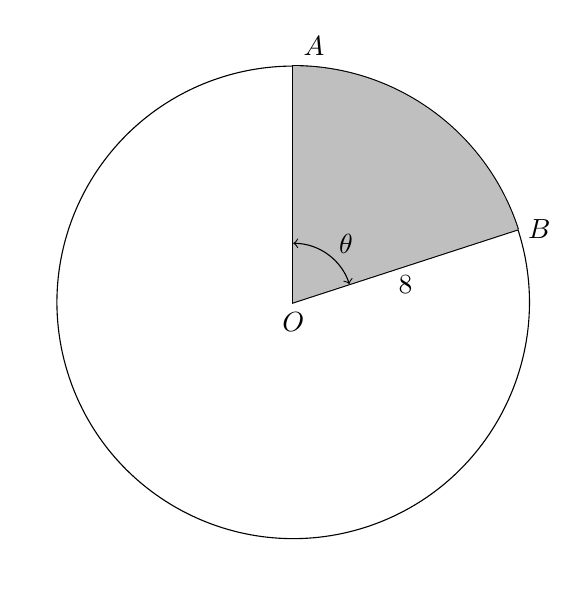
\begin{tikzpicture}[scale=1, rotate=18]
          \draw (0,0) circle[radius=3];
          \draw [thick]
          (0:3) node[right] {$B$}--
          (0,0) node[below] {$O$}--
          (72:3) node[above right] {$A$} arc (72:0:3);
          \fill [lightgray]
          (0,0)--(0:3) arc (0:72:3)--(0,0);
          \draw [<->] (72:0.75) arc (72:0:0.75);
          \node at (30:1){$\theta$};
          \draw (1.5,0) node[below] {$8$};
          %\draw [thick] (0:3)--(72:3)--(2*72:3)--(3*72:3)--(4*72:3)--cycle;
        \end{tikzpicture}
      \end{multicols}  \vspace{3cm}

  \item The coordinates of the vertices of parallelogram $CDEH$ are $C(-5,5)$, $D(2,5)$, $E(-1,-1)$, and $H(-8,-1)$. Find the perimeter of $CDEH$.
    \begin{flushright}
      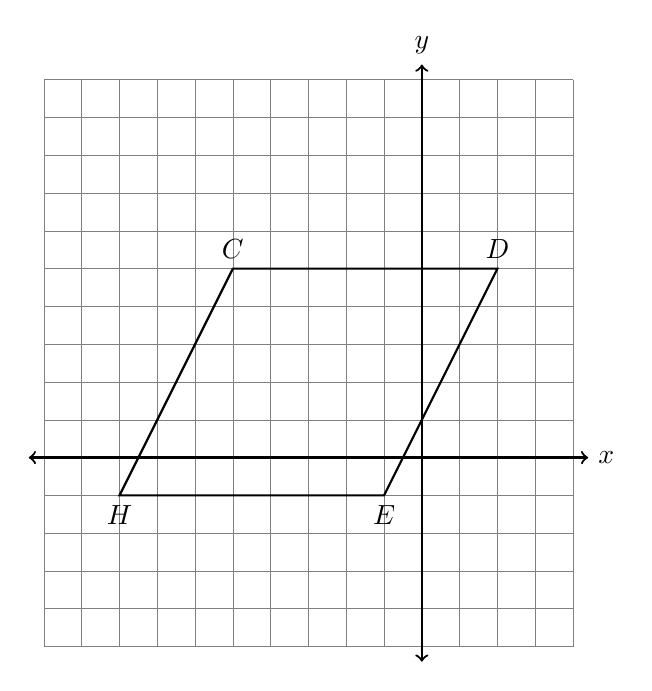
\begin{tikzpicture}[scale=.48]
        \draw [help lines] (-10,-5) grid (4,10);
        \draw [thick, <->] (-10.4,0) -- (4.4,0) node [right] {$x$};
        \draw [thick, <->] (0,-5.4)--(0,10.4) node [above] {$y$};  
        \draw [thick]
          (-5,5) node[above] {$C$}--
          (2,5) node[above] {$D$}--
          (-1,-1) node[below] {$E$}--
          (-8,-1) node[below] {$H$}--cycle;
        %\draw [thick](-5,5)--(-1,-1);
        %\draw [thick](2,5)--(-8,-1);
        %\draw [fill] (-3,2) circle [radius=0.1]node[left]{$P$};
    \end{tikzpicture}
    \end{flushright}

\newpage
\subsubsection*{Vocabulary self-assessment: Circles (fill in the blank with the correct term)}

  \item \textbf{Internal line segments:} Circle with center at point $P$, as shown.
    \begin{multicols}{2}
      \begin{itemize}
        \item  $\overline{AB}$ \quad \rule{3cm}{0.15mm} %Diameter
        \item  $\overline{CP}$ \quad \rule{3cm}{0.15mm} %Radius
        \item  $\overline{DE}$ \quad \rule{3cm}{0.15mm} %Chord
        \item $\angle APC$ \quad \rule{3cm}{0.15mm} %Central angle 
        \item  $\wideparen{AC}$ \quad \rule{3cm}{0.15mm} %(with measure $m\wideparen{AC} = 72^\circ$)Arc
      \end{itemize}
    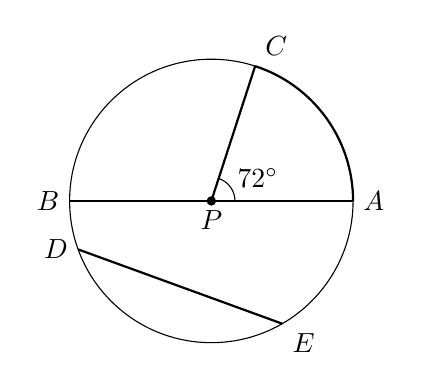
\begin{tikzpicture}[scale=0.6]
      \draw (0,0) circle[radius=3];
      \draw [thick] (3,0) arc (0:72:3);
      \draw [thick] (0:3) node[right] {$A$}--(180:3) node[left] {$B$};
      \draw [thick] (0,0)--(72:3) node[above right] {$C$};
      \draw [thick] (200:3) node[left] {$D$}--(300:3) node[below right] {$E$};
      \fill (0,0) circle[radius=0.1] node[below]{$P$};
      \draw (0.5,0) arc (0:72:0.5) node[right]{$\ 72^\circ$};
      %\draw (35:5) node[right] {$\wideparen{AC}$};
      %\draw (290:5) node[below] {$D$};
    \end{tikzpicture}
  \end{multicols}

  \item \textbf{External lines:} Circle with center at point $O$, at right.
    \begin{multicols}{2}
      \begin{itemize}
        \item  $\overline{FGH}$ \quad \rule{3cm}{0.15mm} %Secant
        \item  $\overline{OJ}$ \quad \rule{3cm}{0.15mm} %Radius
        \item  $\overline{FJK}$ \quad \rule{3cm}{0.15mm} %Tangent
        \item $J$ \quad \rule{3cm}{0.15mm} %Point of tangency 
        %\item Note: $\overline{OJ} \perp \overline{FJK}$
      \end{itemize}
    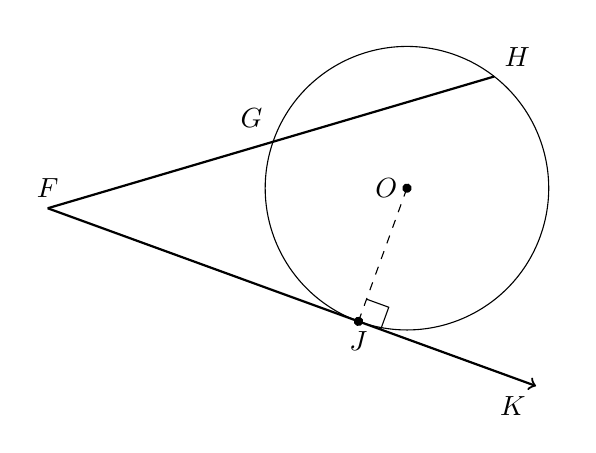
\begin{tikzpicture}[scale=0.6, rotate=-20]
      \draw (0,0) circle[radius=3];
      \draw [thick, ->] (-7,-3) node[above] {$F$}--(4,-3) node[below left] {$K$};
      \draw [thick] (-7,-3)--(72:3) node[above right] {$H$};
      \draw [dashed] (0,-3) node[below] {$J$}--(0,0);
      \fill (0,0) circle[radius=0.1] node[left]{$O$};
      \fill (0,-3) circle[radius=0.1];
      \draw (0,-3) ++(0.5,0)-- ++(0,0.5)--++(-0.5,0);
      \draw (170:3.8) node[below] {$G$};
    \end{tikzpicture}
  \end{multicols}
    
  \item \textbf{Areas:} Circle with center at point $Q$.
    \begin{multicols}{2}
      \begin{itemize}
        \item  $\overline{RS}$ \quad \rule{3cm}{0.15mm} %Diameter
        \item  $RST$ \quad \rule{3cm}{0.15mm} %Semi-circle
        \item  $QUV$ \quad \rule{3cm}{0.15mm} %Sector
      \end{itemize}
    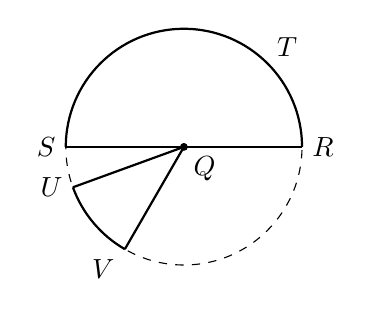
\begin{tikzpicture}[scale=0.5]
      \draw [dashed](0,0) circle[radius=3];
      \draw [thick] (0,0) ++(3,0) arc (0:180:3);
      \draw [thick] (200:3) arc (200:240:3);
      \draw [thick] (0:3) node[right] {$R$}--(180:3) node[left] {$S$};
      \draw [thick] (0,0)--(200:3) node[left] {$U$};
      \draw [thick] (0,0)--(240:3) node[below left] {$V$};
      \fill (0,0) circle[radius=0.1] node[below right]{$Q$};
      \draw (50:3.3) node[right] {$T$};
    \end{tikzpicture}
  \end{multicols}

  \begin{multicols}{2}
  \item \textbf{Polygons and angles in circles:} %Circle with triangle inscribed.
      \begin{itemize}
        \item  $\triangle XYZ$ \vspace{0.5cm} \quad \rule{3cm}{0.15mm} %Inscribed
        \item  $\angle XYZ$ \quad \rule{3cm}{0.15mm} %Inscribed
      \end{itemize} \hspace{1cm}
    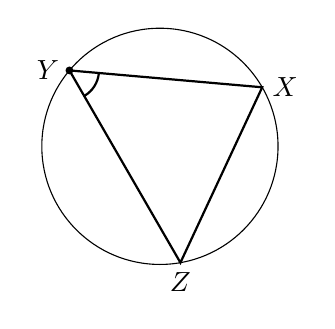
\begin{tikzpicture}[scale=0.5]
      \draw (0,0) circle[radius=3];
      \draw [thick] (140:3) ++(-60:0.75) arc (-60:-5:0.75);
      \draw [thick] (30:3) node[right] {$X$}--(140:3) node[left] {$Y$}
      --(280:3)node[below] {$Z$}--cycle;
      %\draw [thick] (0,0)--(200:3) node[left] {$U$};
      %\draw [thick] (0,0)--(240:3) node[below left] {$V$};
      \fill (140:3) circle[radius=0.1];
      %\draw (50:3.3) node[right] {$T$};
    \end{tikzpicture}
  \end{multicols}

\end{enumerate}
\end{document}
